\documentclass[runningheads,a4paper]{llncs}

\usepackage[T1]{fontenc}
\usepackage[utf8]{inputenc}
\usepackage{graphicx}
\usepackage{booktabs}
\usepackage{multirow}
\usepackage{tabularx}
\usepackage{array}
\usepackage{amsmath}
\usepackage{amssymb}
\usepackage{url}
\usepackage[hidelinks]{hyperref}
\usepackage{microtype}

\newcolumntype{Y}{>{\raggedright\arraybackslash}X}

\begin{document}

\title{Edge--Cloud Reinforcement Learning for Transferable HVAC Control Across Vietnamese Climate Zones}
\titlerunning{Edge--Cloud RL for HVAC Control in Vietnam}

\author{Quoc Hung Nguyen\orcidID{0000-0002-6363-0160}\inst{1}\and
Hoai An Thai\orcidID{0009-0004-4093-522X}\inst{1}\and
Duy Tan Nguyen\orcidID{0009-0000-2832-8647}\inst{1}\and
Vy Le\orcidID{0009-0003-0387-8302}\inst{1}\and
Thi Thuy Duong Nguyen\orcidID{0009-0000-3548-2212}\inst{1}}
\authorrunning{Q. H. Nguyen et al.}

\institute{UEH College of Technology and Design, University of Economics Ho Chi Minh City, Vietnam\\
\email{hungngq@ueh.edu.vn}}

\maketitle

\begin{abstract}
Heating, ventilation, and air-conditioning (HVAC) systems are a major driver of commercial-building electricity use in Vietnam, where a long north--south climate gradient creates a demanding transfer setting for learned controllers. Our focus is not a new PPO variant, but the deployment question: how an HVAC policy should be executed, checked, updated, and transferred across climates. We propose a framework that separates low-latency edge inference from cloud-side multi-context Proximal Policy Optimisation (PPO) retraining. The framework is evaluated with HOT commercial-building archetypes and city-specific TMYx weather files for Ho Chi Minh City, Can Tho, Da Nang, and Hanoi, covering ASHRAE climate zones 0A, 1A, and 2A. The baseline analysis recovers a strong cooling-energy gradient: under identical static setpoints, Ho Chi Minh City consumes $1.44\times$ the HVAC electricity of Hanoi for OfficeSmall and $1.68\times$ for OfficeMedium. Edge inference is approximately $71{,}000\times$ faster than cloud inference at the 95th percentile. Pure-PPO variants reduce comfort violations from $28.7\%$ to $19.8\%$ but increase HVAC energy by $58.7\%$. The proposed edge--cloud controller brings average energy back to within $1\%$ of the static baseline, keeps comfort close to the static baseline, and reduces held-out target energy by $52.0\%$ relative to pure PPO.
\keywords{Reinforcement learning \and HVAC control \and Edge--cloud architecture \and Transfer learning \and Vietnam \and Tropical buildings}
\end{abstract}

\section{Introduction}
Vietnam's commercial-building stock is expanding rapidly, and cooling demand is already a policy-relevant component of national energy use. Reinforcement learning is attractive for HVAC control because it can optimise sequential energy--comfort trade-offs without a hand-derived building model\cite{vazquez2019rl,wang2020review}. However, many HVAC-RL evaluations remain offline and single-climate: they under-report inference latency, climate-driven transfer, and policy-update procedures. These issues are central in Vietnam, whose $\sim 1{,}700$ km north--south gradient spans extremely hot--humid, hot--humid, and warm--humid ASHRAE zones.

The study contributes three elements needed for a deployable HVAC-RL workflow. First, it proposes an edge--cloud architecture in which the edge executes and validates actions while the cloud trains and promotes policy updates. Second, it defines a Vietnam multi-city protocol using HOT building archetypes\cite{berkes2025hot} and EnergyPlus weather data\cite{doe2024epw}. Third, it quantifies a measured energy--comfort trade-off in the Vietnam HOT/EnergyPlus protocol: PPO improves comfort but consumes more energy than static control, whereas the edge--cloud acceptance gate recovers near-static energy use. Code, configurations, trained policies, and aggregated results are released at \url{https://github.com/hoaianthai345/RL_HAVC_Control_VN}.

\section{Related Work}
RL for building control is commonly formulated as a Markov decision process in which observations include thermal state, weather, occupancy, and time features, while actions specify setpoints or actuator commands\cite{vazquez2019rl}. PPO is widely used because its clipped objective improves training stability in continuous control\cite{schulman2017ppo}. Prior work has shown simulation energy savings over fixed or rule-based baselines\allowbreak\cite{zhang2019whole,yu2021review}, but real deployment also requires latency guarantees, safe action validation, and retraining under distribution shift\cite{dulac2021challenges}. Transfer learning for HVAC has been studied across buildings and weather files\cite{fang2023transfer,kadamala2024transfer}; the HOT dataset enables larger-scale cross-climate studies\cite{berkes2025hot}. Edge--cloud AI provides a practical split: latency-sensitive inference stays local, while cloud compute supports retraining and policy governance\cite{shi2016edge,li2023edgeai}.

\section{Methodology}
\subsection{Contextual HVAC Control}
We model each city--building pair $c$ as a contextual MDP $\mathcal{M}_c=\langle\mathcal{S},\mathcal{A},P_c,R_c,\gamma\rangle$. The state contains indoor temperature, outdoor dry-bulb temperature, outdoor relative humidity, occupancy, previous-step HVAC electricity, and time-of-day features. The action is a dual setpoint $a_t=[\mathrm{heat\_sp},\mathrm{cool\_sp}]\in[16,24]\times[20,30]\,^\circ\mathrm{C}$. The reward is
\begin{equation}
 r_t=-\left(0.12e_t+2.0d_t+0.05u_t\right),
\end{equation}
where $e_t$ is 15-min HVAC electricity, $d_t$ is deviation outside the ASHRAE 55 comfort band ($20$--$24\,^\circ\mathrm{C}$)\cite{ashrae55}, and $u_t=\lVert a_t-a_{t-1}\rVert_1$ penalises setpoint chatter.

\subsection{Edge--Cloud Architecture}
Figure~\ref{fig:arch} summarises the proposed architecture. The edge layer executes the 15-min control loop, normalises observations, runs local inference, validates actions against hard bounds and a $1.5\,^\circ\mathrm{C}$ heat--cool separation rule, dispatches setpoints to EnergyPlus, and logs trajectories. The cloud layer aggregates source-context trajectories from Ho Chi Minh City and Can Tho, trains multi-context PPO policies, and promotes a candidate only if a fixed acceptance rule improves energy use without violating comfort-regression, latency, or action-instability constraints. Da Nang and Hanoi are held out from training and used only for transfer evaluation.

\begin{figure}[t]
\centering
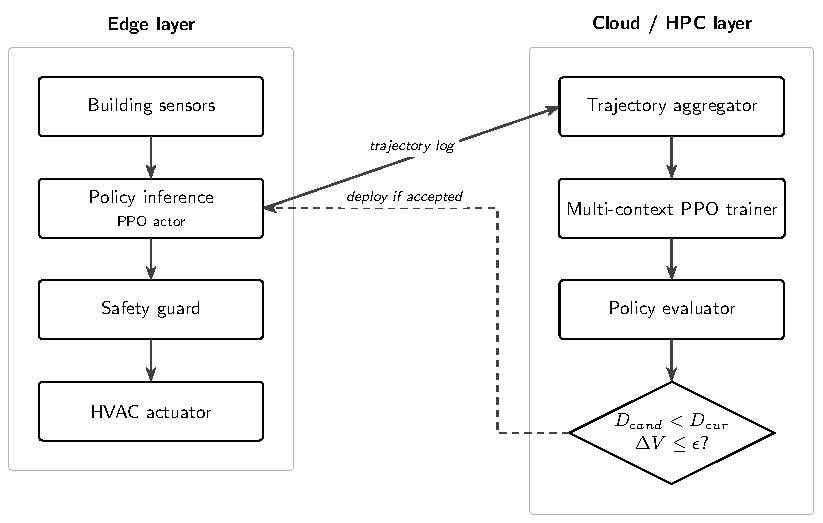
\includegraphics[width=0.90\textwidth]{figures/fig1_architecture.pdf}
\caption{Edge--cloud adaptive RL architecture. Edge devices execute and validate actions; the cloud trains and promotes policy updates.}
\label{fig:arch}
\end{figure}

\section{Experimental Protocol}
\subsection{Cities, Buildings, and Methods}
We use EnergyPlus 24.1 HOT epJSON archetypes calibrated for ASHRAE zone 0A and pair them with city-specific TMYx weather files from Climate OneBuilding\cite{doe2024epw}. The ten evaluated contexts are HCMC and Can Tho (OfficeSmall, OfficeMedium, Hospital) plus Da Nang and Hanoi OfficeSmall/\allowbreak OfficeMedium. HCMC and Can Tho form the source pool; Da Nang and Hanoi are held-out target cities.

We compare seven methods: static setpoints ($20/24\,^\circ\mathrm{C}$), ASHRAE-style outdoor-temperature-conditioned setpoints, a family of single-context PPO checkpoints, multi-context PPO trained jointly on source contexts, edge-only execution of the multi-context policy, cloud-only inference through a safety-aware proxy with simulated network delay ($p_{50}=80$~ms, $p_{95}=85$~ms), and the proposed edge--cloud adaptive controller. PPO uses Stable-Baselines3\allowbreak\cite{stable_baselines3}, $5\times10^5$ timesteps per context, learning rate $5\times10^{-4}$, discount $0.99$, GAE $\lambda=0.95$, clip range $0.15$, and minibatch size 256. Each method is evaluated with three seeds.

\subsection{Metrics}
Control metrics are episode HVAC energy (kWh), comfort-violation rate, mean temperature deviation, cumulative reward, and action instability. Deployment metrics are $p_{50}$/$p_{95}$ inference latency and policy size. Transfer metrics are held-out target energy, target/source energy ratio, adaptation gain, and worst-context energy regret. The results test three hypotheses: H1, static HVAC energy follows Vietnam's north--south climate gradient; H2, edge inference gives a large latency margin; and H3, temperate ASHRAE scheduling does not provide a useful tropical energy--comfort trade-off.

\section{Results}
\subsection{Baseline and Latency Results}
Table~\ref{tab:baselines} supports H1. For OfficeSmall, HCMC consumes $1.44\times$ the static HVAC electricity of Hanoi; for OfficeMedium the ratio is $1.68\times$. Hospitals have near-zero comfort violations but high energy because medical-grade ventilation dominates weather sensitivity. ASHRAE-style scheduling saves energy only by tolerating much higher comfort violation ($80.6\%$ average violation versus $28.7\%$ for static), supporting H3.

\begin{table}[t]
\centering
\caption{Static fixed-setpoint baseline performance (288-step one-day episode; mean over three seeds).}
\label{tab:baselines}
\scriptsize
\begin{tabular}{llrrr}
\toprule
Context & Zone & Energy & Comfort viol. & $\overline{\Delta T}$\\
 & & (kWh) & (\%) & ($^\circ$C)\\
\midrule
HCMC OfficeSmall & 0A & 182.3 & 55.6 & 0.14\\
HCMC OfficeMedium & 0A & 1660.4 & 20.8 & 0.09\\
HCMC Hospital & 0A & 6831.1 & 0.0 & 0.00\\
Can Tho OfficeSmall & 0A & 229.0 & 53.8 & 0.15\\
Can Tho OfficeMedium & 0A & 2480.0 & 18.8 & 0.09\\
Can Tho Hospital & 0A & 6936.6 & 0.0 & 0.00\\
Da Nang OfficeSmall & 1A & 152.4 & 44.4 & 0.11\\
Da Nang OfficeMedium & 1A & 1327.0 & 22.6 & 0.06\\
Hanoi OfficeSmall & 2A & 126.8 & 48.6 & 0.10\\
Hanoi OfficeMedium & 2A & 990.1 & 22.6 & 0.05\\
\bottomrule
\end{tabular}
\end{table}

Table~\ref{tab:latency} supports H2. Edge inference attains $p_{95}=0.00120$ ms, compared with $85.2$ ms for cloud inference, an approximately $71{,}000\times$ latency advantage.

\begin{table}[t]
\centering
\caption{Inference latency over 200 repetitions per context.}
\label{tab:latency}
\begin{tabular}{lrrr}
\toprule
Mode & $p_{50}$ ms & $p_{95}$ ms & Ratio\\
\midrule
Edge-only inference & 0.00119 & 0.00120 & $1\times$\\
Cloud-only inference & 84.4 & 85.2 & $\approx71{,}000\times$\\
PPO checkpoint & \multicolumn{3}{c}{$\sim148$ kB, MlpPolicy with two 64-unit layers}\\
\bottomrule
\end{tabular}
\end{table}

\subsection{PPO Control Performance}
Table~\ref{tab:ppo} shows that pure-PPO policies reduce comfort violations from $28.7\%$ (static) to $19.8\%$, but increase energy from $2091.6$ to $3318.9$ kWh ($+58.7\%$). Under deterministic evaluation, single-context, multi-context, and edge-only PPO converge to identical aggregate rollouts. This equality reflects deterministic evaluation trajectories, not identical checkpoint files or training histories. Cloud-only inference is lower-energy and lower-violation because its safety-aware cloud proxy applies a comfort-priority wrapper when the delay margin is active; this is a deployment-wrapper effect, not a policy-weight effect. The proposed edge--cloud adaptive controller recovers static-level energy ($2072.4$ kWh) and static-level comfort ($26.7\%$ versus $28.7\%$).

\begin{table}[t]
\centering
\caption{Method performance averaged over ten Vietnam contexts.}
\label{tab:ppo}
\small
\begin{tabular}{lrrrr}
\toprule
Method & Energy & Comfort viol. & Reward & Instability\\
 & (kWh) & (\%) & & \\
\midrule
Static setpoint & 2091.6 & 28.7 & $-296.4$ & 0.0035\\
ASHRAE rule-based & 1828.3 & 80.6 & $-1075.7$ & 0.0035\\
Single-context PPO & 3318.9 & 19.8 & $-399.3$ & 0.0174\\
Multi-context PPO & 3318.9 & 19.8 & $-399.3$ & 0.0174\\
Edge-only PPO & 3318.9 & 19.8 & $-399.3$ & 0.0174\\
Cloud-only PPO & 2099.0 & 15.6 & $-285.6$ & 0.0633\\
Edge--cloud adaptive & 2072.4 & 26.7 & $-298.1$ & 0.0608\\
\bottomrule
\end{tabular}
\end{table}

\begin{figure}[t]
\centering
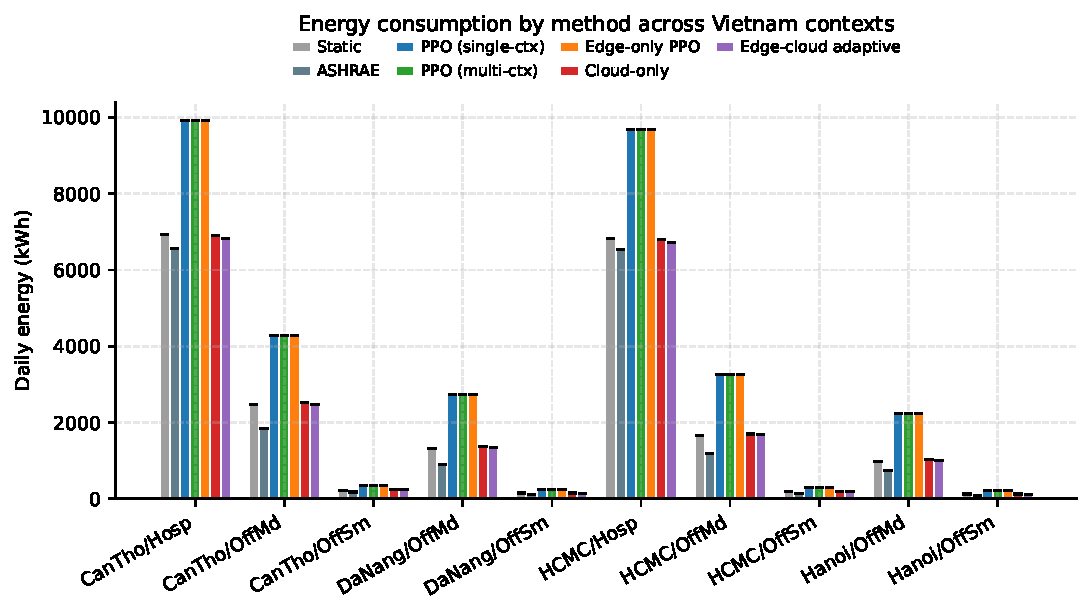
\includegraphics[width=0.48\textwidth]{figures/fig5_energy_by_method.pdf}\hfill
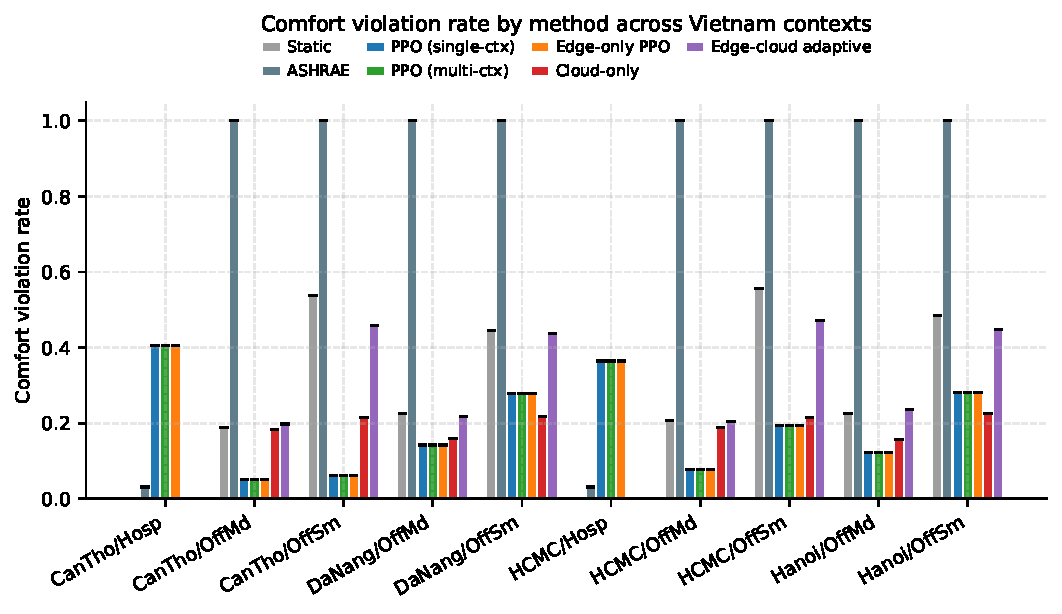
\includegraphics[width=0.48\textwidth]{figures/fig6_comfort_by_method.pdf}
\caption{Per-context energy (left) and comfort-violation rate (right) by control method.}
\label{fig:energy_comfort}
\end{figure}

\subsection{Cross-City Transfer and Adaptation}
Table~\ref{tab:transfer} reports source-domain checks and all four held-out target contexts. The three pure-PPO variants have identical held-out target means ($1358.1$ kWh). The edge--cloud adaptive controller reduces the held-out target mean to $651.7$ kWh, a $52.0\%$ reduction relative to pure PPO. In these rollouts, the gain is therefore attributable mainly to the acceptance layer, since multi-context PPO and single-context PPO produce the same target trajectories.

\begin{table}[t]
\centering
\caption{Transfer energy (kWh). Can Tho is a source-domain check; Da Nang and Hanoi are held-out targets.}
\label{tab:transfer}
\scriptsize
\resizebox{\textwidth}{!}{%
\begin{tabular}{lrrrrrrr}
\toprule
\multirow{2}{*}{Method} & \multicolumn{2}{c}{Can Tho source check} & \multicolumn{4}{c}{Held-out target} & \multirow{2}{*}{Target mean}\\
\cmidrule(lr){2-3}\cmidrule(lr){4-7}
& Sm & Med & Da Nang Sm & Da Nang Med & Hanoi Sm & Hanoi Med & \\
\midrule
Single PPO & 350.6 & 4280.3 & 247.5 & 2724.3 & 217.9 & 2242.9 & 1358.1\\
Multi PPO & 350.6 & 4280.3 & 247.5 & 2724.3 & 217.9 & 2242.9 & 1358.1\\
Edge-only & 350.6 & 4280.3 & 247.5 & 2724.3 & 217.9 & 2242.9 & 1358.1\\
Edge--cloud & 240.1 & 2476.2 & 149.7 & 1333.5 & 124.1 & 999.4 & 651.7\\
\bottomrule
\end{tabular}%
}
\end{table}

Under HCMC AMY weather files for 2022--2024, the adaptation-gain energy delta (TMYx baseline minus AMY mean) is $19.2\pm17.5$ kWh per episode, and comfort-violation rates remain within $\pm3$ percentage points of the TMYx baseline. This indicates robustness to the moderate inter-annual shifts represented by recent HCMC weather years. The deterministic ablation further shows that single-context and multi-context PPO have different checkpoint hashes but indistinguishable aggregate rollouts in this one-day evaluation. Longer stochastic rollouts are needed to isolate regularisation effects.

\section{Discussion and Conclusion}
The experiments indicate that PPO alone is insufficient under the reward weights and one-day evaluation protocol used here. PPO strongly reduces comfort violations but does so by running cooling more aggressively, raising energy by $58.7\%$ over the static baseline. Conversely, ASHRAE-style scheduling reduces energy only by allowing large comfort failures, so it provides no useful tropical energy--comfort advantage. The edge--cloud design separates two operational concerns: edge inference is fast enough for real-time execution, while cloud retraining and acceptance testing provide a practical point at which energy and comfort constraints can be checked before deployment.

The study remains simulation-only. HOT archetypes are calibrated for zone 0A; applying the same models to Hanoi may underestimate winter heating behaviour. All cities share one epJSON per archetype, whereas real buildings vary in envelope, orientation, equipment, and occupancy. The validation also uses one-day episodes; longer stochastic evaluations are required before field deployment.

In summary, Vietnam's multi-zone climate gradient exposes a clear transfer challenge for HVAC control. Pure PPO improves comfort but increases energy, while the proposed edge--cloud adaptive controller achieves near-static energy and comfort and reduces held-out target energy by $52.0\%$ relative to pure PPO. For tropical and warm-humid buildings, the main lesson is that the policy should not be deployed alone: it needs a local safety check and a cloud-side update rule evaluated on target-like weather.

\section*{Acknowledgements}
This research is funded by the University of Economics Ho Chi Minh City (UEH).

\section*{Data Availability}
Building models are drawn from the public HOT dataset\cite{berkes2025hot}. Weather files are from \url{https://climate.onebuilding.org}\cite{doe2024epw}. Code, configuration files, trained policy artifacts, and aggregated result tables are available at \url{https://github.com/hoaianthai345/RL_HAVC_Control_VN}.

\bibliographystyle{splncs04}
\bibliography{references}

\end{document}
